% \documentclass[maturita, czech]{diploma}
% \usepackage{graphicx} % Required for inserting images
% \usepackage{float}
% % \usepackage[czech]{babel}
%
% % \title{manual}
% % \author{konrad.marek }
% % \date{April 2024}
%
%
%
%
%
% \begin{document}
%

\chapter{Uživatelský manuál}

Import naleznete v administraci v boční záložce. 


\section{Import ze školního systému}
V tomto kroku je důležité zvolit správný typ importu.

Tiskové sestavy vygenerujte pomocí rozhraní Bakalářů. Jedná se o sestavy:
\begin{itemize}
    \item \textbf{Seznam předmětů} dle abecedy
    \item \textbf{Úvazky} učitelů s výčtem studentů
    \item \textbf{Seznam skupin} - u všech skupin výčet po řádcích
\end{itemize}
Sestavy nahrajte.

V případě XML importu vyberte vygenerovaný XML soubor.
\begin{figure}[H]
    \centering
    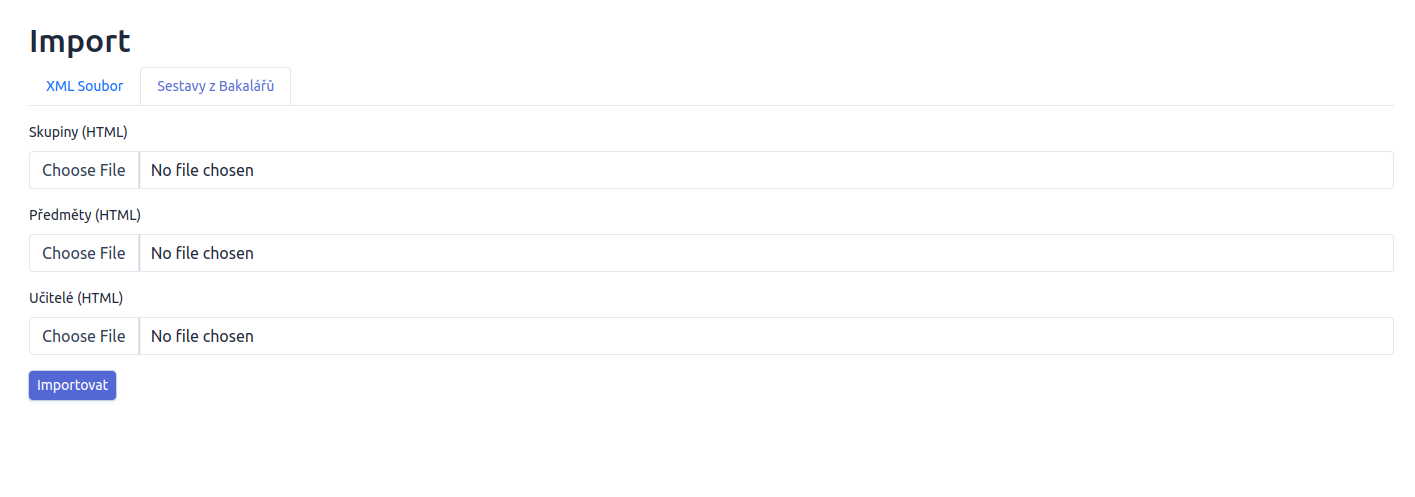
\includegraphics[width=1\linewidth]{Figures/uvodni_import.png}
    \caption{Nahrání sestavy}
    \label{fig:uvodni-import}
\end{figure}
\newpage
\section{Informace o importu}
Tento krok pouze zobrazuje informace o importu ze školního systému.
\begin{figure}[H]
    \centering
    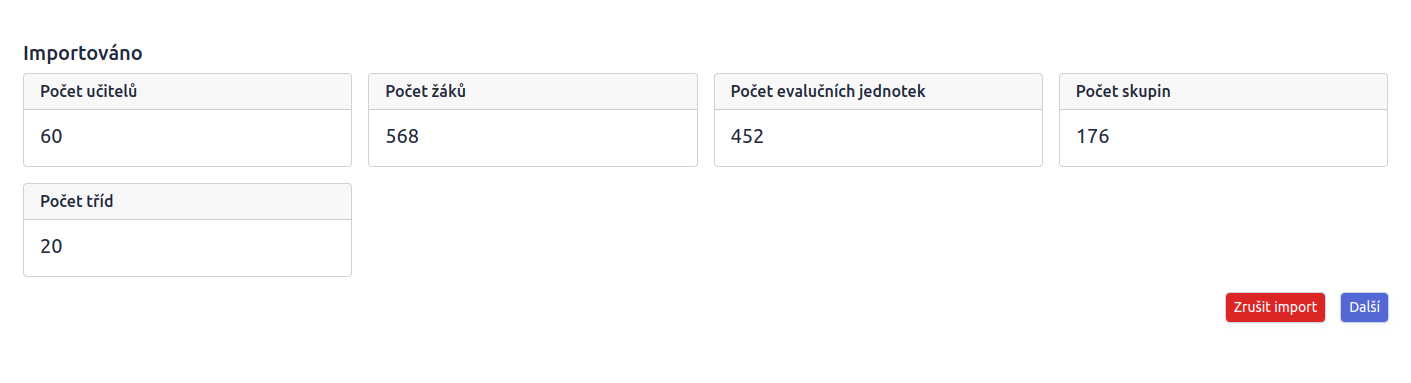
\includegraphics[width=1\linewidth]{Figures/statistika.png}
    \caption{Ukázka informací o importu}
    \label{fig:informace}
\end{figure}

\section{Spojování skupin}
Tento krok je pouze pro import ze sestav.

Jedná se o spojení skupin složených z více tříd. Vyberte kombinaci učitel-předmět a přiřaďte jim skupiny, které se učí spolu. Tlačítkem přidat skupinu naklonujete kombinaci učitel-předmět. Opakujte tento postup dokud nebudete mít vše přiřazeno. Tento krok je nutný, aby úvazky, které jsou učeny zvlášť měly také zvlášť hodnocení.

\begin{figure}[H]
    \centering
    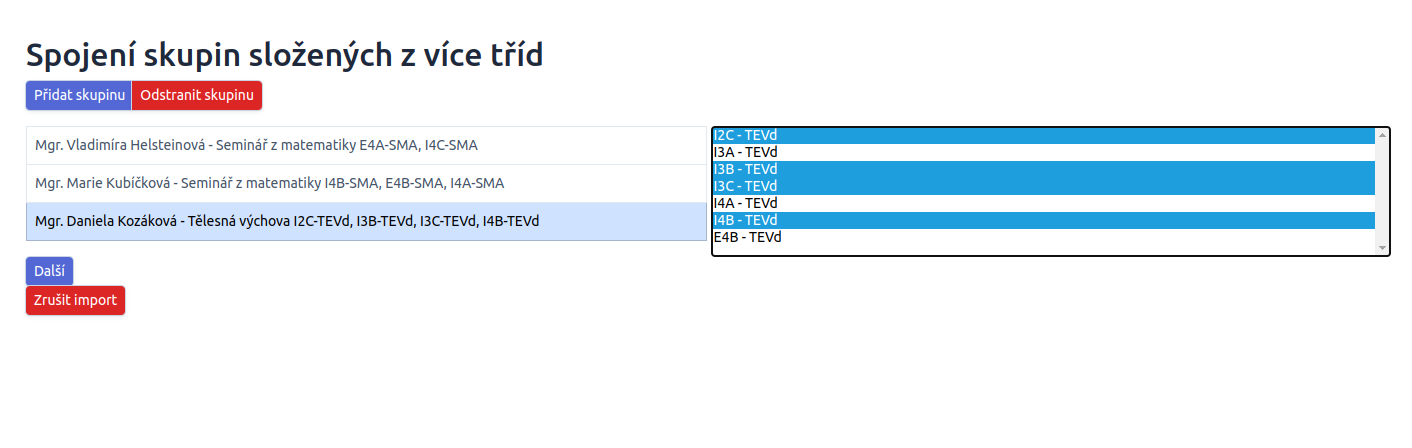
\includegraphics[width=1\linewidth]{Figures/spojovani-skupin.png}
    \caption{Ukázka spojování skupin}
    \label{fig:spojování-skupin}
\end{figure}

\section{Generování emailů}
Pokud nemáte ve školním systému školní emaily žáků bude nutný tento krok. Podobně vypadající krok je i pro generování učitelských emailů. Pro generování emailů se řiďte pokyny aplikace.

\begin{figure}[H]
    \centering
    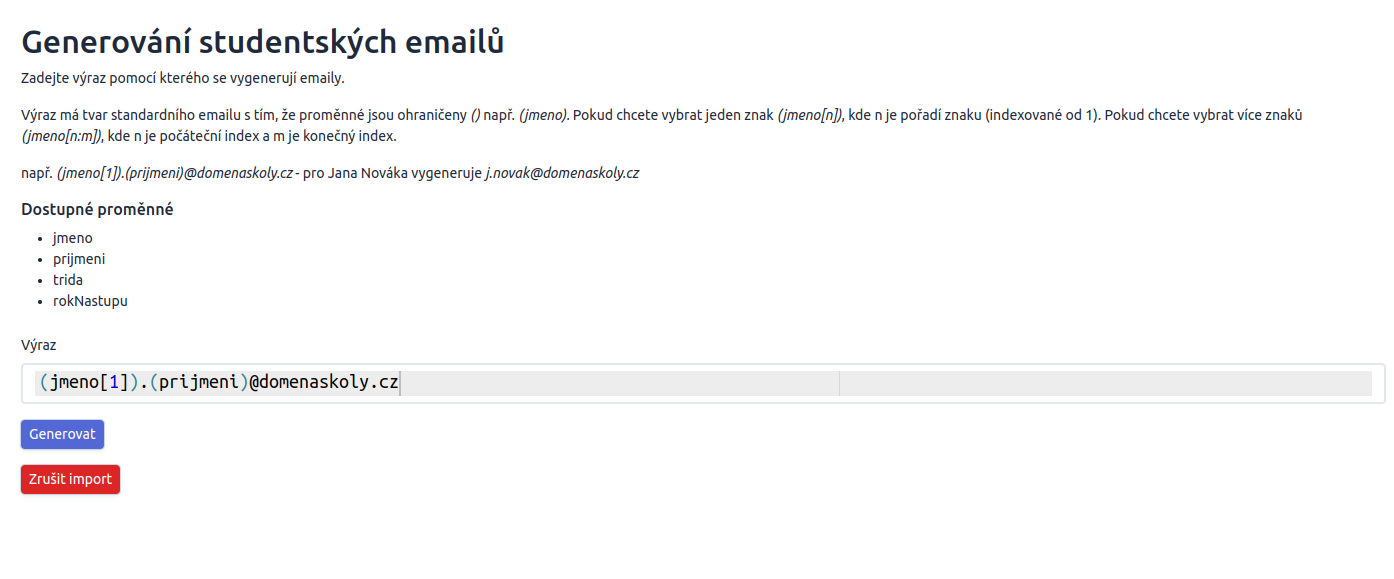
\includegraphics[width=1\linewidth]{Figures/generovani-emailu.png}
    \caption{Ukázka generování emailů}
    \label{fig:generovani-emailu}
\end{figure}


\section{Úprava duplikátních emailů}
Při generování emailů mohlo dojít k vytvoření duplikátů. V tomto kroku se duplikáty odstraní. Ručně přepište emaily žáků.

\begin{figure}[H]
    \centering
    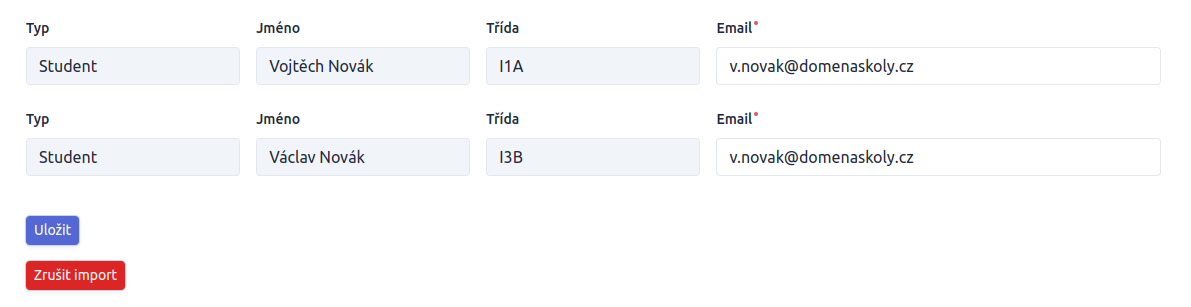
\includegraphics[width=1\linewidth]{Figures/deduplikace.png}
    \caption{Ukázka úpravy duplikátních emailů}
    \label{fig:deduplikace}
\end{figure}


% \end{document}
